% Adapted from the ICASSP 2026 paper
% "Joint Estimation of Piano Dynamics and Metrical Structure with a Multi-task Multi-Scale Network"
% Reorganized for thesis Chapter 5 with minimal technical changes.

\chapter{Audio-to-Score Dynamics via Joint Estimation of Piano Dynamics and Metrical Structure}
\label{ch:audiodyn}

\noindent\textbf{Chapter provenance.}
This chapter is adapted from the ICASSP 2026 paper on joint estimation of piano dynamics and metrical structure. The main architecture, equations, experiments, and quantitative results are retained. The thesis version strengthens the chapter opening, adds task-specific related work, and expands the thesis-facing discussion.

\section{Chapter Overview and Position in the Thesis}
\label{sec:audiodyn:overview}

This chapter addresses the audio-only scenario introduced in Chapter~\ref{ch:introduction}. Unlike the velocity-focused chapters, the target here is not note-level MIDI velocity but beat-synchronous score dynamics. As discussed in Chapter~\ref{ch:background}, score dynamics is human-readable but inherently relative, and its natural coordinate is the beat grid rather than isolated note events. The goal of this chapter is therefore to recover score-level dynamic labels directly from performance audio, while jointly estimating the metrical structure needed to place those labels on a symbolic score.

This chapter occupies a distinct position in the thesis. Chapter~\ref{ch:velcomp} and Chapter~\ref{ch:scoreinf} recover note-level velocity, which is precise and directly editable. The present chapter instead targets a more interpretable score-facing representation. It therefore completes the thesis map by addressing the setting in which audio is the only available input and the desired output is a beat-synchronous symbolic description rather than raw note-level control.

\section{Task-Specific Related Work}
\label{sec:audiodyn:related}

Audio-to-score dynamics recovery is related to, but distinct from, note-level velocity estimation. A large part of the expressive-performance literature studies how performed loudness relates to symbolic dynamic markings and how those markings vary with musical context \cite{kosta2014dynpiano,kosta2016mapping,jones2023probingdyn}. This literature makes two points that matter here. First, score dynamics is musically meaningful and worth recovering. Second, it is inherently ambiguous and cannot be reduced to a fixed physical threshold.

A second relevant line of work concerns metrical structure estimation. Beat and downbeat tracking has a strong literature in MIR, with modern deep models achieving increasingly robust results \cite{bock2020deconstruct,zhao2022beat,foscarin2024beat}. For the present chapter, beat and downbeat estimation is not only an auxiliary task. It is part of the output interface because score dynamics is easiest to interpret and evaluate on a beat grid.

These observations motivate a joint rather than isolated formulation. Predicting score dynamics without metre produces labels that are hard to place. Predicting metre without dynamics misses the expressive target. The present chapter therefore studies score-facing dynamics recovery through joint estimation of dynamic levels, change points, beats, and downbeats.

\section{Problem Setting and Targets}
\label{sec:audiodyn_targets}

Chapter~\ref{ch:background} already introduced the ambiguity of score dynamics, the distinction between score dynamics and MIDI velocity, and the role of beats and downbeats as a musically meaningful coordinate. Rather than repeat that background, this chapter focuses on the concrete transcription problem studied in this work.

Given a piano performance audio signal, the system predicts four synchronized output sequences on a frame grid: dynamic levels, dynamic change points, beats, and downbeats. The dynamic targets are the score-facing outputs, while beats and downbeats provide the metrical structure required to align these labels to a symbolic score. This joint design serves two practical modes of use. In the first mode, a reliable beat grid is already available from an aligned score or a score-level AMT system, and the predicted dynamic labels are attached to that grid. In the second mode, no score is available, and the model first predicts beats and downbeats by itself, then uses the estimated grid to place the dynamic labels.

More specifically, the dynamic-level target is formulated as a six-class frame-wise prediction problem, including one \textit{blank} class before the first annotated marking and the five score-dynamics classes used in MazurkaBL: \textit{pp}, \textit{p}, \textit{mf}, \textit{f}, and \textit{ff}. The change-point target is binary and indicates whether a contextual transition between adjacent dynamic regimes occurs at a given time. Beats and downbeats are also binary frame-wise targets. At inference time, the frame-wise outputs are converted into beat-synchronous score annotations by sampling the dynamic class at beat locations and snapping detected change points to the nearest beat.

\begin{figure}[t]
  \centering
  \IfFileExists{Chapter_5/figures/p1.png}{%
    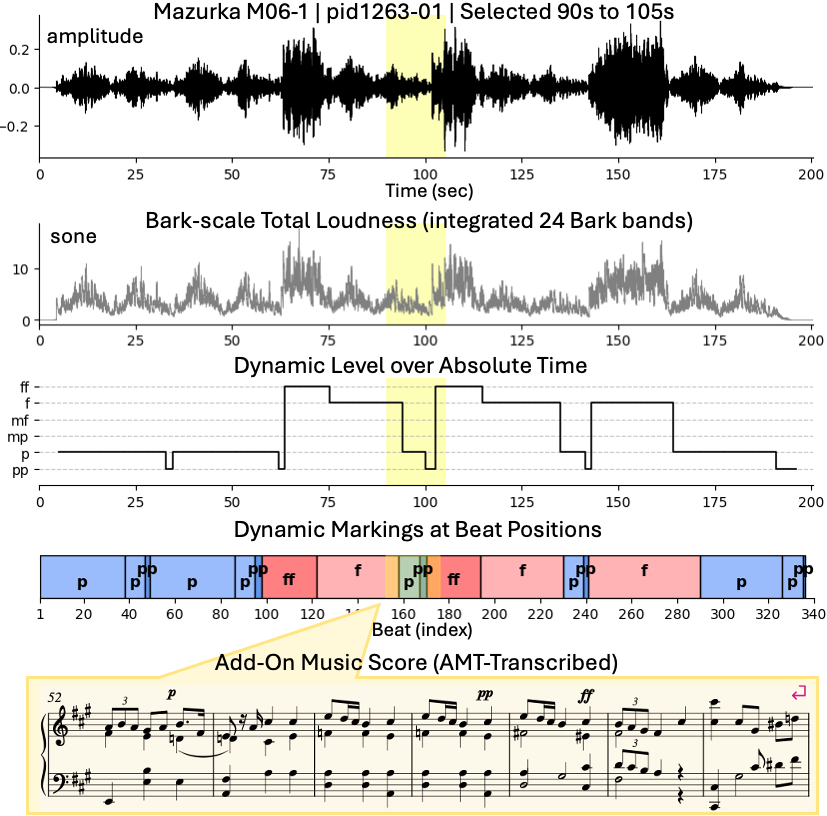
\includegraphics[width=0.95\textwidth]{Chapter_5/figures/p1.png}%
  }{%
    \fbox{\parbox{0.92\textwidth}{\vspace{4.8cm}\centering\textit{Placeholder for workflow figure from the ICASSP paper. Replace with \texttt{Chapter\_5/figures/p1.png}.}\vspace{4.8cm}}}%
  }
  \caption{Workflow for adding dynamic markings to an AMT-transcribed score from audio. The highlighted region (90--105 s of Chopin Mazurka Op.~6 No.~1) shows a case study. Dynamic markings are aligned with the musical beat grid, and a change point indicates a contextual shift in the dynamic levels.}
  \label{fig:audiodyn_workflow}
\end{figure}

This task directly matches the role assigned to Chapter~5 in the thesis plan: score-level dynamics should be represented as a beat-synchronous interface comprising dynamic levels, change points, and metrical structure. It also supports the broader thesis objective of recovering expressive labels without changing the underlying note content or timing.

\section{Perceptually Grounded Features and Multi-Scale Backbone}
\label{sec:audiodyn_features}

\subsection{Bark-scale specific loudness}
\label{ssec:audiodyn_bssl}

Chapter~\ref{ch:background} established the psychoacoustic chain behind BSSL: physical level is measured in dB, frequency-dependent loudness level is expressed in phons, perceptual magnitude is expressed in sones, and the spectral distribution of that perceptual magnitude is organized on the Bark scale rather than on raw FFT bins. For the present chapter, the important point is that BSSL is not merely a compressed spectrogram. It is a sampled representation of \emph{specific loudness} across auditory critical bands, and therefore explicitly models the fact that neighbouring spectral components interact through critical-band integration and spectral masking \cite{zwicker1999psychoacoustics,pampalk2002content,kosta2017thesis}. The conceptual motivation is given in Chapter~\ref{ch:background}; here we restate the operational part of that formulation because it directly determines the front-end used by the model.

In continuous psychoacoustic notation, specific loudness is written as $N'(z,t)$, where $z$ denotes critical-band rate in Bark. In the discrete MIR front-end used here, we work with Bark-wise samples $N'_b(t)$, one value per auditory band. As recalled from Chapter~\ref{ch:background}, the Bark coordinate is obtained from physical frequency $f$ through a mapping such as
\begin{equation}
z(f)=13\arctan(0.76 f_{\mathrm{kHz}})+3.5\arctan\!\left(\frac{f_{\mathrm{kHz}}^2}{7.5^2}\right),
\label{eq:audiodyn_bark_mapping}
\end{equation}
where $f_{\mathrm{kHz}}$ denotes frequency in kHz \cite{pampalk2002content,pampalk2004exploring,zwicker1999psychoacoustics}. This reparameterization matters because loudness summation is constrained by critical-band structure: energy falling inside the same auditory band does not contribute independently, and a strong component can partially mask nearby components.

Operationally, the short-time power spectrum $P(k,t)$ is first weighted by an outer- and middle-ear transfer approximation, then grouped into Bark bands, and finally passed through a spreading operation that models spectral masking across neighbouring bands. Writing $A_{\mathrm{dB}}(f)$ for the auditory weighting term and $G(\cdot)$ for the spreading function, the front-end can be summarized as
\begin{equation}
E_b(t)=\sum_{k\in\mathcal{B}_b} P(k,t)\,10^{A_{\mathrm{dB}}(f_k)/10},
\qquad
\widetilde{E}_b(t)=\sum_{i=1}^{B} E_i(t)\,10^{G(b-i)/10},
\label{eq:audiodyn_spread}
\end{equation}
where $\mathcal{B}_b$ is the set of FFT bins associated with Bark band $b$ \cite{terhardt1979outerear,schroeder1979masking,pampalk2002content}. This is the implementation-facing version of the argument made in Chapter~\ref{ch:background}: if score dynamics is linked to perceived intensity, then the front-end should not treat each narrowband magnitude as perceptually independent. The weighting and spreading stages yield a Bark-domain excitation pattern that is closer to human loudness perception than raw spectral magnitude alone.

The resulting Bark-domain excitation is then converted from loudness level to sones. Using the same phon-to-sone mapping introduced in Chapter~\ref{ch:background} (cf. Eq.~\eqref{eq:bg:sone_from_phon}), the specific loudness in band $b$ at frame $t$ is
\begin{equation}
N'_b(t)=
\begin{cases}
2^{(L_N(b,t)-40)/10}, & L_N(b,t)\ge 40,\\[4pt]
\left(L_N(b,t)/40\right)^{2.642}, & L_N(b,t)<40,
\end{cases}
\label{eq:audiodyn_specific_loudness}
\end{equation}
where $L_N(b,t)$ denotes the Bark-band loudness level in phons \cite{bladon1981vowel,kosta2017thesis,narang2024automatic}. The matrix $\mathbf{X}=[N'_b(t)]$ is what we call BSSL in this chapter. By contrast, Bark-scale total loudness would collapse this distribution to a single scalar,
\begin{equation}
N_{\mathrm{tot}}(t)\approx \sum_{b=1}^{B} N'_b(t)\,\Delta z_b,
\label{eq:audiodyn_total_loudness}
\end{equation}
which corresponds to the relation between specific loudness and total loudness already discussed conceptually in Chapter~\ref{ch:background}. That scalar is useful for visualization, smoothing, or change-point inspection, but it is not used as model input here. For score-dynamics estimation it matters not only how much loudness is present overall, but also how that loudness is distributed across register and spectral balance. Two excerpts can have similar total loudness and still differ substantially in the Bark-wise pattern that a listener hears.

Bark-scale features are therefore a natural fit for the present task. While log-Mel spectrograms remain dominant in modern deep learning pipelines, the effectiveness of Bark-based representations is supported by extensive research. For instance, recent work has demonstrated that Bark-scale cepstral coefficients can improve speaker recognition under short-duration constraints \cite{zi2024bgcc}, and a high-resolution variant of BSSL has shown performance gains over log-Mel inputs for vocal dynamics estimation \cite{narang2024automatic}. Given the growing evidence supporting Bark-scale features, coupled with BSSL's established success in previous piano dynamics research \cite{kosta2016mapping}, we adopt it as the foundational feature for this work.

The primary challenge was the implementation of the BSSL extractor. Standardized toolboxes like MOSQITO \cite{san2021mosqito}, while compliant with ISO 532-1:2017, are designed for robust sound-quality assessment and therefore mandate a 48~kHz sampling rate with constrained STFT parameters. Since most music and piano recordings are encoded at 44.1~kHz, using MOSQITO would require upsampling, which is computationally expensive and can introduce interpolation artifacts. We therefore implemented a custom BSSL extractor in PyTorch by reproducing the \texttt{ma\_sone} function from the widely used Music Analysis MATLAB toolbox by Pampalk \cite{pampalk2004toolbox}, which is based on the algorithmic chain proposed in \cite{pampalk2002content}. This implementation gives the parameter flexibility needed for fair and efficient experimentation.

The feature extraction pipeline begins by converting audio to mono and peak-normalizing it to $-1$~dBFS. To ensure compatibility with a recent state-of-the-art beat tracking model \cite{foscarin2024beat}, the audio is resampled to 22.05~kHz, and a short-time Fourier transform is computed using a Hann window of length 1024 and a frame rate of 50~fps. The resulting power spectrogram is then transformed into BSSL through the psychoacoustic stages summarized above: outer- and middle-ear weighting, grouping into critical bands, spectral spreading, and nonlinear mapping to the perceptual \textit{sone} scale. This yields the final input feature matrix $\mathbf{X} \in \mathbb{R}^{22 \times T}$, where $T$ is the number of frames. The choice of 22 Bark bands is determined by the 11.025~kHz Nyquist frequency, which fully covers the 22nd Bark band. While integrated loudness is convenient for visualization, the full $22 \times T$ BSSL matrix is used as model input in order to preserve the Bark-wise specific-loudness structure motivated in Chapter~\ref{ch:background}.

\subsection{Shared multi-scale encoder}
\label{ssec:audiodyn_encoder}

A central modeling challenge is that the four tasks do not require the same temporal context. Dynamic estimation requires a large temporal receptive field \cite{narang2024automatic}, whereas beat and downbeat tracking require high temporal resolution to localize transient onsets \cite{bock2020deconstruct}. To reconcile these conflicting requirements, we adapt the multi-scale network of \cite{li2023frame} as a shared encoder.

Given an $F \times T$ time--frequency feature as input, the feature map is first normalized with 2D batch normalization. The encoder then processes three parallel branches at temporal resolutions $T$, $T/s$, and $T/s^{2}$, where the scaling factor $s$ controls the amount of downsampling and upsampling. Each branch is built from residual blocks and self-attention blocks following \cite{li2023frame}. In contrast to the original single-task formulation, we treat $s$ as a tunable hyperparameter and let the encoder output a shared latent sequence $\mathbf{Z} \in \mathbb{R}^{T \times 8}$ for subsequent multi-task decoding.

\begin{figure}[t]
  \centering
  \IfFileExists{Chapter_5/figures/p2.png}{%
    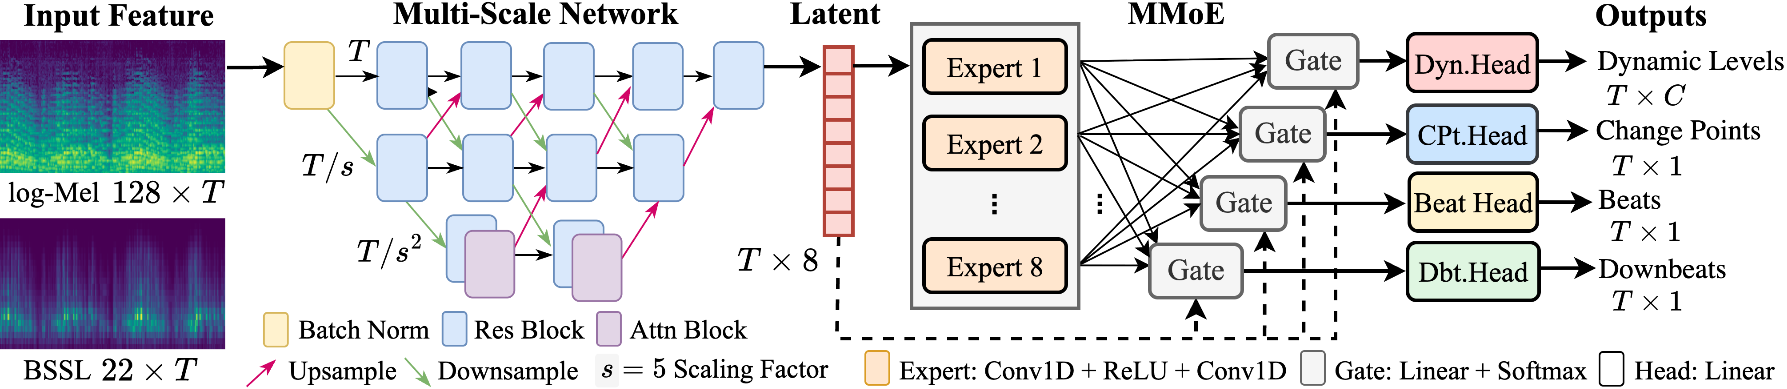
\includegraphics[width=\textwidth]{Chapter_5/figures/p2.png}%
  }{%
    \fbox{\parbox{0.95\textwidth}{\vspace{4.4cm}\centering\textit{Placeholder for architecture figure from the ICASSP paper. Replace with \texttt{Chapter\_5/figures/p2.png}.}\vspace{4.4cm}}}%
  }
  \caption{Architecture of the proposed multi-task framework. A three-branch multi-scale network encodes either log-Mel or BSSL input. Branches operate at lengths $T$, $T/s$, and $T/s^{2}$, with outputs a latent sequence of shape $T\times8$. An 8-expert MMoE with four gates forms task-specific features, followed by linear heads to output four distinct targets. The scaling factor $s$ is a tunable hyperparameter.}
  \label{fig:audiodyn_model}
\end{figure}

The use of BSSL is especially important in this architecture because input dimensionality directly affects parameter count. The compact 22-band input permits substantially longer audio segments than a 128-bin log-Mel front-end, which is important for phrase-level dynamic context and is later confirmed by the ablation study.

\section{Joint Estimation with Task-Aware Decoding}
\label{sec:audiodyn_mtl}

\subsection{MMoE decoder}
\label{ssec:audiodyn_mmoe}

The shared encoder provides a common latent representation, but the tasks remain acoustically diverse. To reduce negative transfer, we use a Multi-gate Mixture-of-Experts (MMoE) layer \cite{ma2018mmoe} as a task-aware decoder.

The MMoE module contains a pool of eight shared experts. Each expert is a lightweight temporal convolutional block with two sequential 1D convolutional layers of kernel size 3 and length-preserving padding, separated by a ReLU activation. All experts process the shared latent sequence $\mathbf{Z}$ in parallel.

For each task $k$, a dedicated gating network $G_k(\cdot)$ acts as a dynamic router. At time step $t$, the gate takes the latent feature $\mathbf{z}_t$ and outputs a softmax-normalized weight vector $\mathbf{w}_k(t) \in \mathbb{R}^{8}$. The task-specific feature vector is then computed as a weighted combination of expert outputs:
\begin{equation}
\mathbf{y}_{k,t} = \sum_{i=1}^{8} \mathbf{w}_{k,i}(t) \cdot \mathbf{e}_{i,t},
\qquad
\mathbf{w}_k(t) = \operatorname{Softmax}(G_k(\mathbf{z}_t)).
\label{eq:audiodyn_mmoe}
\end{equation}
Here, $\mathbf{e}_{i,t}$ is the output of expert $i$ at time step $t$. Repeating this process frame by frame yields the task-specific sequence $\mathbf{Y}_k = [\mathbf{y}_{k,1}, \dots, \mathbf{y}_{k,T}]^{\top} \in \mathbb{R}^{T \times 8}$, which is then mapped to logits by a separate linear head for each task.

\subsection{Task-specific post-processing}
\label{ssec:audiodyn_post}

The model outputs frame-wise probabilities, which are converted into discrete musical events through tailored post-processing. For beat and downbeat detection, we adopt the post-processing procedure from \cite{foscarin2024beat}: probabilities are thresholded at 50\%, and peak picking is applied within a 70~ms neighborhood ($\pm 3$ frames at 50~fps). For dynamic markings, the dynamic level at each detected beat is determined by taking the \texttt{argmax} of the class probabilities at that frame.

Change points are determined in two stages. First, we identify all frames whose change-point probability exceeds 75\%. Second, we snap each candidate to the nearest detected beat. This beat-snapping step is motivated by the annotation style of MazurkaBL, where dynamic markings are beat-aligned rather than freely placed in continuous time \cite{kosta2018mazurkabl}. The step also keeps evaluation consistent with prior work \cite{kosta2017thesis}.

\subsection{Loss function}
\label{ssec:audiodyn_loss}

Training uses a composite multi-task objective,
\begin{equation}
\mathcal{L}_{\mathrm{MTL}} =
\mathcal{L}_{\mathrm{Dyn}} +
\mathcal{L}_{\mathrm{CPt}} +
\mathcal{L}_{\mathrm{Beat}} +
\mathcal{L}_{\mathrm{Dbt}}.
\label{eq:audiodyn_loss}
\end{equation}
For the binary targets (change points, beats, and downbeats), we use the shift-tolerant weighted binary cross-entropy proposed in \cite{foscarin2024beat}. This loss addresses two difficulties at once: the target sequences are extremely sparse, and the annotations can contain small timing imprecision. For the multiclass dynamic-level target, we use standard cross-entropy masked by the ground-truth beat positions. This mask imposes a data-driven prior that reflects the annotation style of MazurkaBL, namely that dynamic markings occur only on beats, and suppresses spurious inter-beat fluctuations.

\section{Experimental Setup}
\label{sec:audiodyn_exp}

\subsection{Dataset and protocol}
\label{ssec:audiodyn_data}

We use the MazurkaBL dataset \cite{kosta2018mazurkabl}, a score-aligned corpus of 2{,}098 solo piano recordings covering 44 Chopin Mazurkas. After excluding two mazurkas with irregular dynamics annotations (M06-4 and M63-2), 1{,}999 recordings are used. Although newer datasets such as EME33 \cite{hung2024eme33} exist, MazurkaBL remains the largest publicly available resource for studying notated dynamics against performed loudness from audio. Its provision of score-aligned beat times and verified expressive markings makes it particularly suitable for the task of beat-synchronous score-dynamics transcription.

We use 5-fold cross-validation stratified by mazurka. For each fold, the model is trained for 120 epochs, and the best checkpoint is selected on the validation set using F1 score. Optimization uses AdamW with learning rate $3 \times 10^{-4}$, batch size 10, and fixed random seed 86.

During training, audio is sliced into 60-second segments with 50\% overlap. No overlap is used at evaluation time. Both BSSL and log-Mel features are extracted with the same STFT configuration to ensure identical temporal resolution. The empirically optimal temporal scaling factor is $s=5$. The model predicts six dynamic classes: one \textit{blank} class and the five annotated dynamic levels \textit{pp}, \textit{p}, \textit{mf}, \textit{f}, and \textit{ff}. On an NVIDIA RTX~3090 (24~GiB), a full 5-fold run requires approximately 20 hours, with peak GPU memory usage around 4~GiB.

\subsection{Baselines}
\label{ssec:audiodyn_baselines}

We compare the proposed model against both single-task baselines and task-specific baselines.

\paragraph{Single-task multi-scale network.}
We establish single-task baselines by adapting the multi-scale network from \cite{li2023frame}, integrating its public implementation into our data pipeline, and training one independent model per target. Each single-task model uses the corresponding task-specific loss from the multi-task objective, with scaling factor $s=5$.

\paragraph{Dynamic and change-point baselines.}
For dynamics and change points, we report published results from representative methods in \cite{kosta2017thesis}, namely the Artificial Neural Network (ANN) for dynamics and the Pruned Exact Linear Time (PELT) algorithm for change-point detection. These methods are tuning-intensive and not end-to-end, so we report their published scores rather than re-implementing them.

\paragraph{Beat and downbeat baselines.}
For beats and downbeats, we include the time-convolutional network with dynamic Bayesian network post-processing \cite{bock2020deconstruct} and the recent state-of-the-art transformer model Beat This \cite{foscarin2024beat}. Both models are retrained from scratch on MazurkaBL using their public code and the same 5-fold protocol as ours.

\subsection{Evaluation metrics}
\label{ssec:audiodyn_metrics}

All four tasks are evaluated using F1 score. For beat and downbeat tracking, we report F1 with a $\pm 70$~ms tolerance, following \cite{bock2020deconstruct,foscarin2024beat}. Dynamics and change points follow the evaluation protocol of \cite{kosta2017thesis}. For dynamics, the continuous dynamic-level output is sampled at each ground-truth beat location, discretized into score markings, and evaluated using macro-averaged F1 over the five dynamic classes \textit{pp}, \textit{p}, \textit{mf}, \textit{f}, and \textit{ff}, excluding the \textit{blank} class. For change points, predictions are snapped to the nearest ground-truth beat before F1 evaluation. This turns both dynamics and change-point evaluation into a beat-wise comparison on a musically meaningful grid.

\section{Results, Case Study, and Discussion}
\label{sec:audiodyn_results}

\begin{table}[t]
\centering
\caption{Performance comparison of the proposed model against all baselines. Per-task F1 scores (\%) are reported as mean $\pm$ standard deviations over 5-fold cross-validation. PELT is an algorithmic method with no trainable parameters, while ANN did not report this attribute. The best score in each column is highlighted in bold.}
\label{tab:audiodyn_main_results}
\begingroup
\fontsize{10pt}{10pt}\selectfont
\setlength{\tabcolsep}{3pt}
\renewcommand{\arraystretch}{1.2}
\begin{tabular}{l l c c c c r}
\toprule
Method & Feature & Dynamic & Change Point & Beat & Downbeat & \# Params \\
\midrule
ANN \cite{kosta2017thesis} & BSSL & 29.4 & -- & -- & -- & n/a \\
PELT \cite{kosta2017thesis} & BSSL & -- & 10.8 & -- & -- & n/a \\
TCN+DBN \cite{bock2020deconstruct} & log-Mel & -- & -- & $60.9 \pm 1.8$ & $30.4 \pm 1.3$ & 0.1 M \\
Beat This \cite{foscarin2024beat} & log-Mel & -- & -- & $80.5 \pm 2.7$ & $52.8 \pm 6.2$ & 20.3 M \\
\midrule
Single-task Multi-scale & BSSL & $50.6 \pm 10.1$ & $21.0 \pm 9.9$ & $84.0 \pm 1.5$ & $45.0 \pm 1.7$ & 0.4 M \\
\quad w/o. BSSL & log-Mel & $50.4 \pm 11.1$ & $17.5 \pm 5.4$ & $83.8 \pm 1.8$ & $54.7 \pm 7.5$ & 13.3 M \\
\midrule
Multi-task Multi-scale & BSSL & \textbf{$54.4 \pm 8.9$} & \textbf{$26.1 \pm 9.7$} & \textbf{$84.1 \pm 1.3$} & $55.2 \pm 4.2$ & 0.5 M \\
\quad w/o. BSSL & log-Mel & $50.8 \pm 10.9$ & $23.1 \pm 6.1$ & $83.7 \pm 1.7$ & \textbf{$58.5 \pm 6.2$} & 14.7 M \\
\bottomrule
\end{tabular}

\endgroup
\end{table}

\subsection{Main results}
\label{ssec:audiodyn_mainres}

Table~\ref{tab:audiodyn_main_results} shows that the proposed multi-task framework gives the strongest overall results on MazurkaBL. With BSSL input, it achieves the best scores for dynamics, change points, and beats, while the log-Mel variant of the same framework achieves the best downbeat F1. The BSSL configuration is therefore the best overall trade-off, and it is the configuration adopted as the main system in this chapter.

The multi-task formulation is consistently better than the corresponding single-task counterpart under the same BSSL front-end. Relative to the single-task BSSL model, the proposed multi-task model improves dynamic F1 by 3.8 points, change-point F1 by 5.1 points, beat F1 by 0.1 points, and downbeat F1 by 10.2 points. These gains indicate that joint learning is useful rather than harmful in this setting, provided that the shared representation is combined with task-aware decoding.

The feature comparison also reveals an important trade-off. BSSL is better for dynamics, change points, and beats, whereas log-Mel remains slightly better for downbeats. The practical advantage of BSSL lies in its compactness: the input dimensionality drops from 128 mel bins to 22 Bark bands, reducing the model size from 14.7~M parameters to 0.5~M in the multi-task setting. This drastic reduction enables much longer input sequences and makes long-context training feasible on modest hardware.

This result should not be read as a dimensionality effect alone. In the terms of Chapter~\ref{ch:background}, BSSL preserves the Bark-wise distribution of specific loudness after auditory weighting and masking, whereas a scalar loudness curve would discard that structure and a conventional log-Mel spectrogram does not encode it explicitly. The gains in dynamic and change-point prediction are therefore consistent with the thesis-level claim that score-dynamics recovery benefits from a representation closer to perceived loudness than to raw spectral magnitude.

\begin{table}[t]
\centering
\caption{Ablation study of the multi-task network with BSSL features. Per-task F1 scores (\%, mean over 5 folds) and their arithmetic average are reported.}
\label{tab:audiodyn_ablation}
\begingroup
\fontsize{9pt}{11pt}\selectfont
\setlength{\tabcolsep}{4pt}
\renewcommand{\arraystretch}{1.0}
\begin{tabular}{l c c c c c}
\toprule
Setting & Dyn F1 & CPt F1 & Bt F1 & Dbt F1 & Average \\
\midrule
Proposed & \textbf{54.4} & \textbf{26.1} & \textbf{84.1} & \textbf{55.2} & \textbf{55.0} \\
\quad w/o. MMoE & 52.8 & 22.0 & 82.9 & 51.8 & 52.4 \\
\quad w/o. Temp. Scal. & 50.5 & 13.3 & 80.3 & 41.9 & 46.5 \\
\quad w/o. Data Augm. & 50.5 & 19.6 & 83.2 & 51.7 & 51.2 \\
\quad uses 30s Segment & 49.1 & 19.2 & 83.4 & 52.7 & 51.1 \\
\bottomrule
\end{tabular}
\endgroup
\end{table}

\subsection{Ablation study}
\label{ssec:audiodyn_ablation}

To validate the design choices, we conduct four ablations against the full BSSL model: removing MMoE, disabling temporal scaling by setting $s=1$, removing overlap-based data augmentation, and shortening the audio segment from 60 seconds to 30 seconds. Table~\ref{tab:audiodyn_ablation} shows that all four choices matter. The largest drop is caused by removing temporal scaling, which confirms that the task combination genuinely benefits from multi-scale context. Removing MMoE also causes a clear degradation, which supports the claim that task-aware routing mitigates negative transfer.

The 60-second input length is especially important for the dynamics-related tasks. Compared with the 30-second setting, the full model improves dynamic F1 from 49.1 to 54.4 and change-point F1 from 19.2 to 26.1. This supports the main modeling intuition of the chapter: phrase-level dynamic context extends well beyond the shorter windows commonly used in beat tracking.

\subsection{Case study and interpretability}
\label{ssec:audiodyn_case}

Figure~\ref{fig:audiodyn_workflow} illustrates how the model output can be turned into score-level annotations. The highlighted excerpt shows a piecewise-constant dynamic trajectory aligned to beat positions, while a detected change point marks a contextual shift between local dynamic regimes. This qualitative example is important because the objective of the chapter is not continuous loudness tracking for its own sake. The aim is to produce labels that can be written back onto a score or compared on a common beat grid across performances.

This beat-synchronous interface also improves interpretability. Dynamic levels provide a compact symbolic summary, while change points explain where that summary changes. Beats and downbeats make the output musically navigable. Together, the four targets form a practical bridge between raw audio and human-readable score annotations.

\subsection{Discussion: why score dynamics is not a relabelled MIDI velocity problem}
\label{ssec:audiodyn_discussion}

This chapter makes a different thesis-level point from Chapters~\ref{ch:velcomp} and \ref{ch:scoreinf}. The target is not note-level control, and the output is not intended to drive a synthesizer directly. Instead, the objective is a score-facing summary of expressive intensity on a musically meaningful coordinate. Score dynamics is therefore not obtained here by simply discretizing an underlying velocity curve. It is learned as a symbolic description of dynamic regimes together with the metrical structure needed to place that description on a score.

This distinction explains several design choices. The model uses longer context because phrase-level dynamic intent extends beyond local note attacks. The post-processing snaps change points to beats because the available annotations are editorial and metrical rather than freely continuous. The evaluation is beat-synchronous because a musically meaningful score label should be judged on the score grid, not only on raw frame precision.

The chapter also complements Thread~A rather than replacing it. Note-level velocity is the more precise target when the goal is editing or rendering. Beat-synchronous score dynamics is the more interpretable target when the goal is symbolic annotation, educational feedback, or performance analysis. The thesis requires both views in order to connect machine-readable control with human-readable musical description.

% ===== THESIS TODO (recommended final addition) =====
% Add one richer case study from MazurkaBL that shows an editorially ambiguous passage.
% Suggested thesis-facing conclusion: the model can recover musically plausible dynamic regimes,
% but disagreement between score editions and annotation conventions limits any single-label ceiling.

\subsection{Limitations}
\label{ssec:audiodyn_limits}

Several limitations should be kept in mind. First, the dynamic vocabulary is restricted to the five static score levels present in MazurkaBL plus a \textit{blank} class. The model does not explicitly represent longer-span symbols such as \textit{crescendo} and \textit{diminuendo}; instead, it captures local transitions through change points. Second, the beat-aligned post-processing reflects the annotation style of MazurkaBL. This is musically sensible for this dataset, but it may not transfer directly to corpora with different editorial conventions.

Third, the experiments are limited to solo piano recordings, and the repertoire is concentrated on Chopin mazurkas. The chapter therefore demonstrates that audio-to-score dynamics transcription is feasible in a controlled but musically meaningful setting, rather than claiming immediate generalization to other instruments or styles. Finally, the feature comparison suggests that no single front-end is uniformly optimal across all tasks: BSSL is the better global choice for the present chapter, but downbeat tracking still benefits from log-Mel input.

\section{Summary}
\label{sec:audiodyn_summary}

This chapter established a compact multi-task, multi-scale framework for recovering beat-synchronous score dynamics directly from piano audio. Using Bark-scale specific loudness as input and MMoE as task-aware decoding, the model jointly predicts dynamic levels, change points, beats, and downbeats while remaining highly parameter-efficient. On MazurkaBL, the framework achieves strong benchmark results and shows that long-context, perceptually grounded audio modeling is a practical route from performance audio to score-level dynamic annotations. Within the broader thesis, this chapter provides the Thread~B counterpart to the velocity-focused methods of the preceding chapters, addresses Requirement~R4 most directly through its beat-synchronous output design, and completes the audio-only scenario of expressive label recovery.